\documentclass[fontsize=11pt]{article}
\usepackage{amsmath}
\usepackage[utf8]{inputenc}
\usepackage[margin=0.75in]{geometry}
\usepackage{graphicx}
\usepackage{hyperref}

\renewcommand{\baselinestretch}{1.25}

\title{CSC111 Project Proposal: BUILDING A CHECKERS AI PLAYER}

\author{Sujoy Deb Nath, Benjamin Lee, Mohamed Abdullahi and, Eren Findik}
\date{Tuesday, March 16, 2021}

\begin{document}
\maketitle

\section*{Problem Description and Research Question}

$~~~~$Over the past few decades, the use of technology has become more prevalent and mainstream. Along with this increase in technological innovation, the use of artificial intelligence has also been on the rise. Computers being able to think and makes decisions is a very interesting field, and something that everyone in our group is interested in. Thus, we have decided to pursue AI development for our final project. More specifically, we want to build an AI that plays checkers. \\

Checkers is an old game that that was invented c. 3000 B.C.E (Gamesver Team, 2020), with multiple variations and play styles across different regions of the world. Overall, it is a well-known and widely played game. Checkers is a fairly complex game, but a few things remain constant across most variations. There are two sides/players, black and white, and the main win condition is that one side has captured/removed all of the opponent’s pieces. In this case, we mean that when a piece is captured, it is removed from the board. We will explain more about which board style and rules we will follow for this project later down below. The main idea here is that if removing all of the opponent’s pieces counts towards victory, and preserving your own pieces counts towards survival, then we want to find out if \textbf{tracking the average number of pieces each player could potentially lose when making a move is a good indicator of win probability \textsl{(i.e. can the AI win games more often than if it made decisions randomly and can it do well against an actual player)}?}

\subsection*{What is Simplified Checkers?}

$~~~~$Now before going any further, it would be good to have an understanding of our version of checkers. As stated before, checkers is a fairly complex game with multiple variations, thus we have built our own simplified version of checkers based on North American checkers. \\

North American checkers has an 8 x 8 board with 12 white and 12 black pieces (Ultraboardgames.Com, 2021). The arrangement of the board below:

$$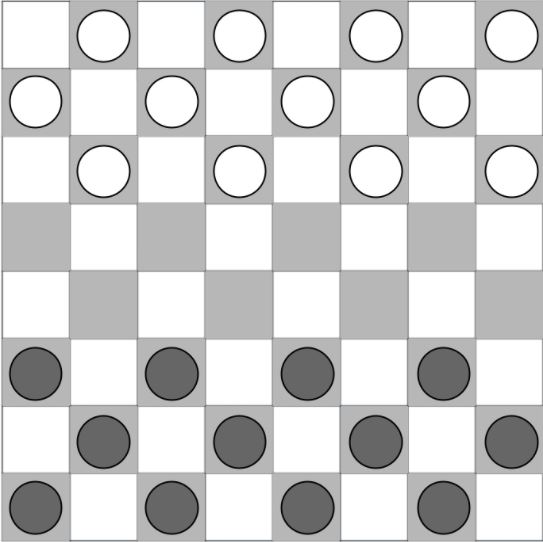
\includegraphics[width=6cm]{normal_checkers.JPG}$$

We are concerned that implementing and creating the full game of checkers, along with creating an AI might be impossible for us to complete by the deadline, thus we decided to create a simplified version of checkers. Our version has a 6 x 6 board with 6 pieces per player.

$$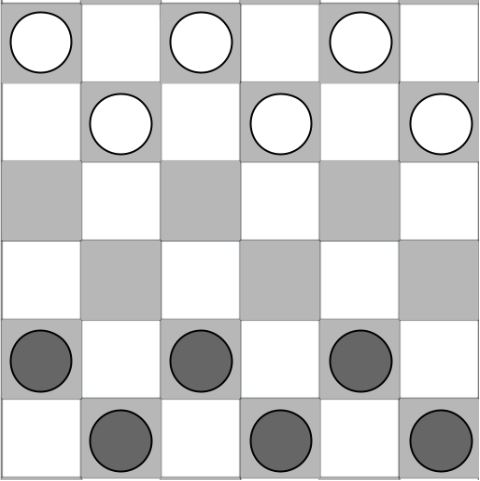
\includegraphics[width=6cm]{simplified_checkers.JPG}$$

Reducing the board size and the number of pieces reduces the computation time, complexity, and the number of possible moves and games. If our simplified version of checkers still proves to be too difficult, we will add the additional restriction of no multiple jumps/captures per move.  

\section*{Computational Plan}

\subsection*{Building Checkers in Python}

$~~~~$There will be 3 classes: Piece, which will be used to represent each counter/piece on the checkers board, Checkers, which represents the game itself, and Player, which will include the AI’s or the actual humans that make the moves. The piece class will keep track of the color (boolean), position (string), and whether it's a king (boolean) of the piece. Checkers class will keep track of the board (list of Pieces), players (Player type), moves played (A doubly linked list), the whether the game has ended (boolean) and the number of moves (int). A move will be represented as a tuple of 3 strings. Where the first string is the initial position, the second is optional and would be the position of the piece it attacks, and the third is the final position. The game ends when a total number of possible moves is reached or one side loses all its pieces. If the game is ended, then it disables any further moves, but enables the user to see which moves are played throughout the game.


\subsection*{Using the Tree data type to build a GameTree}

$~~~~$In order to record the possible moves our AI can make, we would use the tree data type. Each node in the tree would contain a specific move and the number of pieces both players could potentially lose (the number of pieces of each player will be a different attribute).\\

$~~~~$The way we make our game tree will be similar to how it was made in assignment 2. We will store all the past games in a csv file and use a method similar to \texttt{insert\_move\_sequences} in assignment 2 to create a game tree from the csv file. Every time a game is played, we will add the sequence of moves to a csv file. 

\subsection*{Creating an AI that uses a Game Tree}

$~~~~$In checkers, the number of pieces a player has usually matters the most. For that reason, rather than building an AI player that uses win probability to make its decisions, we will instead build an AI that tracks the number of pieces lost by each color and makes decisions based on that. \\

Our AI player will have two variations, aggressive player and defensive player. For the aggressive AI player, it will not care about the number of pieces it will lose and it will pick its next move based on only the number of pieces its opponent will lose. When the Aggressive AI player makes its next move, it will choose the subtree with highest number of pieces lost by its opponent. In contrast, the defensive AI player will try to preserve as many of its pieces as possible and choose its next move based on the number of pieces it will lose.\\

We will also construct an Exploring AI that will initially make random moves to explore all the possible moves and build a Gametree. Essentially, the Exploring player will try to pick moves that don't exist in the game tree (i.e. have never been played before). We could then make the Aggressive AI player or the Defensive AI player use that Gametree by storing the Gametree in a CSV file or in a variable and then pass it to either of the AI’s parameters as an argument.


\subsection*{Representing Checkers Visually using Pygame}

$~~~~$First, the board is going to be built using two nested for loops. Then, with two separate for loops, the pieces will be added to a board. One for loop will draw the white pieces, and the other one will draw the black pieces using \texttt{pygame.draw.circle()}. So far, we have created the initial position of the board before the start of the game. After the game starts, the board will be updated in every move by \texttt{make\_move()} function -if an opponent’s piece is taken, it will disappear, and the piece that the player moves will be transported to the new square.\texttt{time.sleep() }in the time module will be used to create delays in the game, so that people can see the motion of the pieces. If the player is an actual human, then his moves will be kept track of by mouse events. (Pygame.mouse, 2020)\\

\subsection*{Reporting Results}

We would show the results by showing statistics through simulations of games played and by allowing people to interact with the chess AIs. The statistics will be similar to how win percentages were shown in assignment 2. We would run simulations with the different AIs and see how they do against each other. We plan on allowing people to play against the different AI’s so that they would be able to determine how good they are.

\section*{References}

\begin{itemize}
    \item Gamesver Team. “History of Checkers - Easily Explained (with Pictures).” Gamesver, Ropcaf, 25 Jan. 2020,
    \url{www.gamesver.com/history-of-checkers-easily-explained-with-pictures/}. 
    
    \item "How To Play Checkers | Official Rules | Ultraboardgames". Ultraboardgames.Com, 2021,
    
    \url{https://www.ultraboardgames.com/checkers/game-rules.php}.
    
    \item Pygame. Pygame.draw - Pygame v2.0.1.dev1 Documentation, Nov. 2020, 
    \url{www.pygame.org/docs/ref/draw.html}. 

    \item Pygame. Pygame.mouse - Pygame v2.0.1.dev1 Documentation, Nov. 2020, 
    
    \url{www.pygame.org/docs/ref/mouse.html}.

    \item Time - Time Access and Conversions - Python 3.9.2 Documentation, 
    
    \url{docs.python.org/3/library/time.html#time.sleep}.

\end{itemize}
% NOTE: LaTeX does have a built-in way of generating references automatically,
% but it's a bit tricky to use so we STRONGLY recommend writing your references
% manually, using a standard academic format like APA or MLA. https://owl.purdue.edu/owl/research_and_citation/apa_style/apa_formatting_and_style_guide/general_format.html)
% (E.g., 

\end{document}
